\section{Date: 2026-08-16}
\noindent \textbf{Series ID: PCU517311517311111} 

\noindent This series is titled Producer Price Index by Industry: Wired Telecommunications Carriers: Residence Local Telephone Service and has a frequency of Monthly. The units are Index Dec 2003=100 and the seasonal adjustment is Not Seasonally Adjusted.The observation start date is 1995-06-01 and the observation end date is 2026-07-01.The popularity of this series is 1. \\ 

\noindent \textbf{Series ID: WFRBSDEN09} 

\noindent This series is titled Share of Deposits Held by the 90th to 99th Wealth Percentiles and has a frequency of Quarterly. The units are Percent of Aggregate and the seasonal adjustment is Not Seasonally Adjusted.The observation start date is 1989-07-01 and the observation end date is 2026-01-01.The popularity of this series is 3. \\ 

\subsection{Raw Regression}
\noindent Regresses the two series against each other directly. A significant result here can come just as easily from both series sharing a long-run trend as from any real relationship.

\begin{center}
\begin{tabular}{lclc}
\toprule
\textbf{Dep. Variable:}                  & value\_fred\_WFRBSDEN09 & \textbf{  R-squared:         } &     0.118   \\
\textbf{Model:}                          &           OLS           & \textbf{  Adj. R-squared:    } &     0.111   \\
\textbf{Method:}                         &      Least Squares      & \textbf{  F-statistic:       } &     16.27   \\
\textbf{Date:}                           &     Sun, 16 Aug 2026    & \textbf{  Prob (F-statistic):} &  9.68e-05   \\
\textbf{Time:}                           &         12:14:37        & \textbf{  Log-Likelihood:    } &   -261.14   \\
\textbf{No. Observations:}               &             123         & \textbf{  AIC:               } &     526.3   \\
\textbf{Df Residuals:}                   &             121         & \textbf{  BIC:               } &     531.9   \\
\textbf{Df Model:}                       &               1         & \textbf{                     } &             \\
\textbf{Covariance Type:}                &        nonrobust        & \textbf{                     } &             \\
\bottomrule
\end{tabular}
\begin{tabular}{lcccccc}
                                         & \textbf{coef} & \textbf{std err} & \textbf{t} & \textbf{P$> |$t$|$} & \textbf{[0.025} & \textbf{0.975]}  \\
\midrule
\textbf{const}                           &      32.1950  &        0.816     &    39.451  &         0.000        &       30.579    &       33.811     \\
\textbf{value\_fred\_PCU517311517311111} &       0.0260  &        0.006     &     4.033  &         0.000        &        0.013    &        0.039     \\
\bottomrule
\end{tabular}
\begin{tabular}{lclc}
\textbf{Omnibus:}       & 15.062 & \textbf{  Durbin-Watson:     } &    0.016  \\
\textbf{Prob(Omnibus):} &  0.001 & \textbf{  Jarque-Bera (JB):  } &   17.361  \\
\textbf{Skew:}          &  0.918 & \textbf{  Prob(JB):          } & 0.000170  \\
\textbf{Kurtosis:}      &  3.127 & \textbf{  Cond. No.          } &     561.  \\
\bottomrule
\end{tabular}
%\caption{OLS Regression Results}
\end{center}

Notes: \newline
 [1] Standard Errors assume that the covariance matrix of the errors is correctly specified.

\begin{figure}
\centering
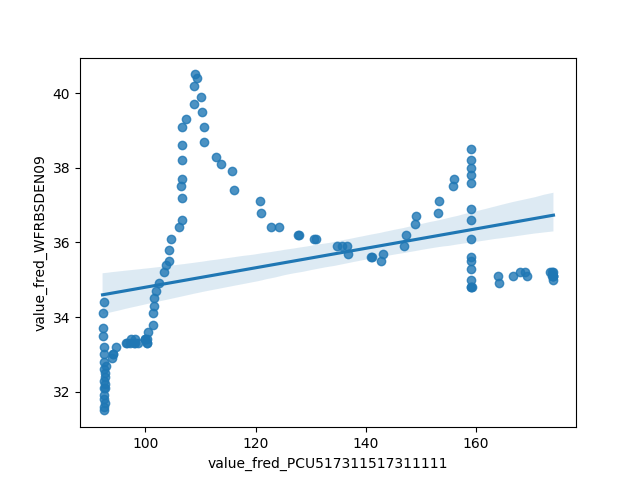
\includegraphics[scale = 0.9]{plots/plot_2026-08-16.png}
\caption{Raw Regression Plot for 2026-08-16}
\end{figure}
\newpage
\subsection{Detrended Regression}
\noindent Regresses the residuals of each series after removing its own linear time trend, so a shared trend can no longer drive the result on its own. A relationship that stays significant here is better evidence of a genuine link between the two series.

\begin{center}
\begin{tabular}{lclc}
\toprule
\textbf{Dep. Variable:}                             & value\_fred\_WFRBSDEN09\_detrended & \textbf{  R-squared:         } &     0.406   \\
\textbf{Model:}                                     &                OLS                 & \textbf{  Adj. R-squared:    } &     0.401   \\
\textbf{Method:}                                    &           Least Squares            & \textbf{  F-statistic:       } &     82.82   \\
\textbf{Date:}                                      &          Sun, 16 Aug 2026          & \textbf{  Prob (F-statistic):} &  2.24e-15   \\
\textbf{Time:}                                      &              12:14:38              & \textbf{  Log-Likelihood:    } &   -217.79   \\
\textbf{No. Observations:}                          &                  123               & \textbf{  AIC:               } &     439.6   \\
\textbf{Df Residuals:}                              &                  121               & \textbf{  BIC:               } &     445.2   \\
\textbf{Df Model:}                                  &                    1               & \textbf{                     } &             \\
\textbf{Covariance Type:}                           &             nonrobust              & \textbf{                     } &             \\
\bottomrule
\end{tabular}
\begin{tabular}{lcccccc}
                                                    & \textbf{coef} & \textbf{std err} & \textbf{t} & \textbf{P$> |$t$|$} & \textbf{[0.025} & \textbf{0.975]}  \\
\midrule
\textbf{const}                                      &    5.594e-13  &        0.129     &  4.33e-12  &         1.000        &       -0.256    &        0.256     \\
\textbf{value\_fred\_PCU517311517311111\_detrended} &      -0.1489  &        0.016     &    -9.100  &         0.000        &       -0.181    &       -0.116     \\
\bottomrule
\end{tabular}
\begin{tabular}{lclc}
\textbf{Omnibus:}       & 13.682 & \textbf{  Durbin-Watson:     } &    0.048  \\
\textbf{Prob(Omnibus):} &  0.001 & \textbf{  Jarque-Bera (JB):  } &   15.396  \\
\textbf{Skew:}          &  0.841 & \textbf{  Prob(JB):          } & 0.000454  \\
\textbf{Kurtosis:}      &  2.578 & \textbf{  Cond. No.          } &     7.90  \\
\bottomrule
\end{tabular}
%\caption{OLS Regression Results}
\end{center}

Notes: \newline
 [1] Standard Errors assume that the covariance matrix of the errors is correctly specified.

\begin{figure}
\centering
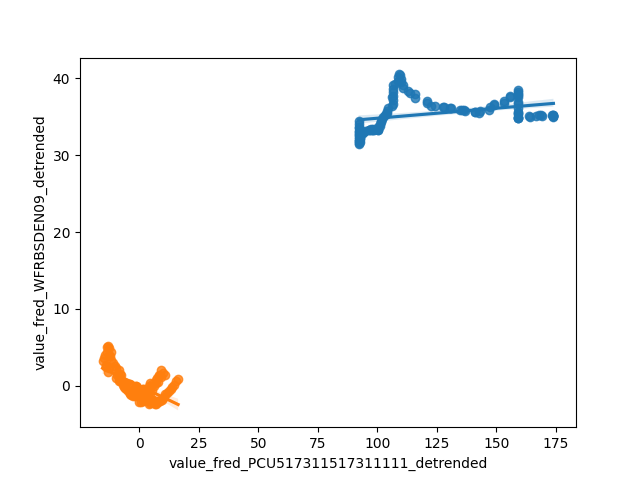
\includegraphics[scale = 0.9]{plots/plot_2026-08-16_detrended.png}
\caption{Detrended Regression Plot for 2026-08-16}
\end{figure}
\newpage
